\ifx
\begin{figure}[htbp]
\centering
\subfigure[Focus point Suggestion]{
	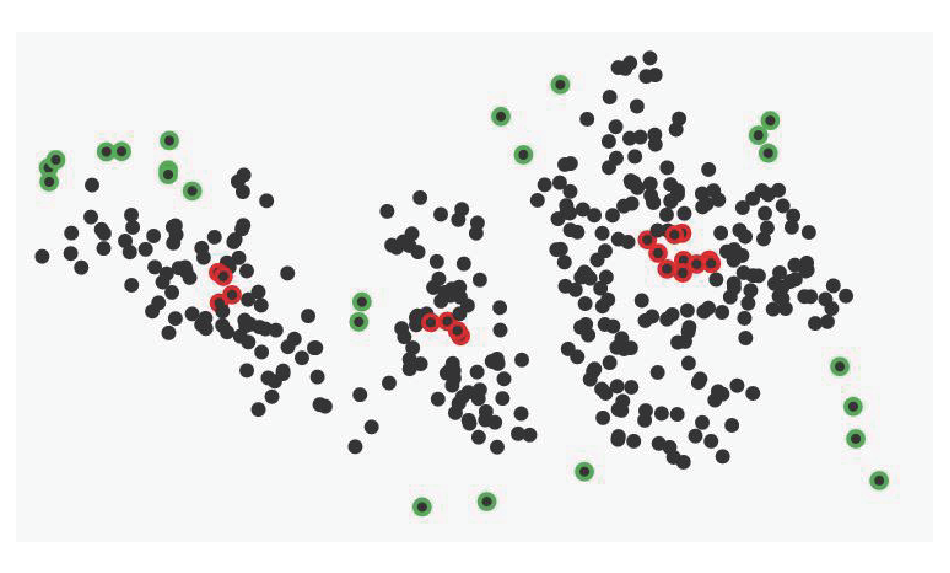
\includegraphics[width=0.48\linewidth]{images/suggestion_point_new.eps}
}
\subfigure[Focus Group Suggestion]{
	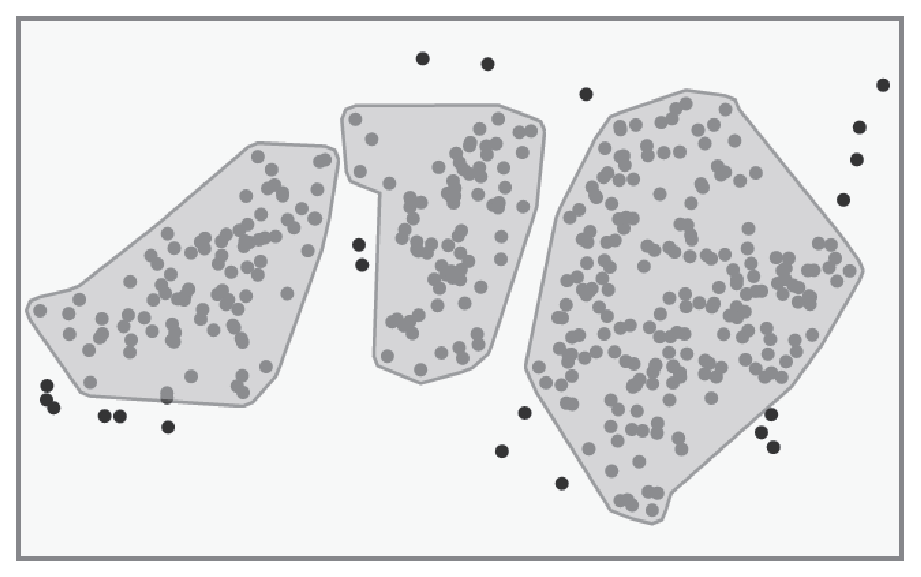
\includegraphics[width=0.46\linewidth]{images/suggestion_group_new.eps}
}
  \caption{Focus Suggestion: We provide}
\label{fig:suggestions}
  \end{figure}
  \else
\begin{figure}[htbp]
\centering
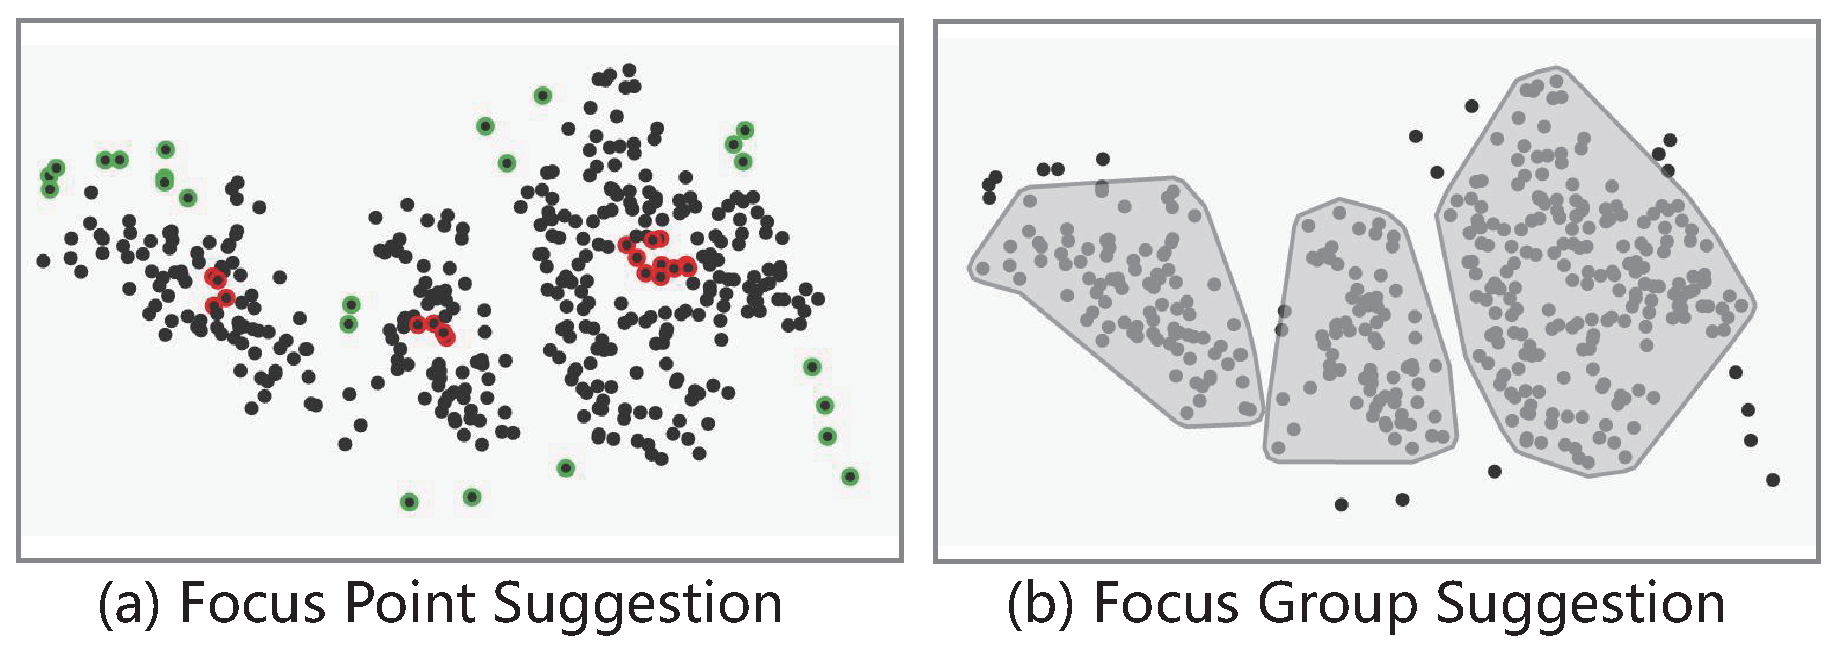
\includegraphics[width=1\linewidth]{images/suggestion_new.eps}
  \caption{Focus Suggestions. (a) Representative points (red) and outliers (green) are recommended as potential POI points. (b) Clusters are revealed in the projection, guiding users to choose a proper POI group.}
\label{fig:suggestions}
\end{figure}
  \fi
\section{High-dimensional Local Data Analysis in Locally Enhanced Projections}
As stated before, our method supports a four-step exploration. In this section, we'll introduce in detail how we support this POI-based exploration in each step.
\label{section:method}
\subsection{Discovering Interesting Local Focus}
Shneiderman has suggested in his information seeking mantra~\cite{DBLP:conf/vl/Shneiderman96}: "Overview first, then detail on demand". Following the suggestion, we first provide a PCA projection as an overview of the data. Users can brush any part of the data they feel interesting and claim it as a focus. However, it may not be easy for users who have no analytic backgrounds or prior knowledge about the data. Hence, we also recommend to users some potential focuses generated via automatic detection algorithms. Different suggestions are made for different types of POIs (point or group).

Note that, we make all recommendations based on the projected data, i.e. a distorted copy, rather than the original high-dimensional data. There are two reason for such practice. Firstly, no additional or prior knowledge should be assumed in a free exploration. Users choose their focuses based on what they perceive. Therefore, we should also recommend based on what is presented to users. Secondly, the locally enhanced projections are capable of revealing underlying data features. What's been misunderstood due to distortions can be corrected in the POI-enhanced layouts. By changing the focus, users can gradually clarify data structures in different local regions.
\note{
In a projection, there are two situations where some local data is considered interesting. The first case is about distance distortion. Incorrect distances result in false neighborhoods. Closely distributed data in the projection may be far away in the original space and vice versa. Data involved in a distorted local area is regarded informative in the projection. It's also the basic idea in previous works concerning about data locality~\cite{DBLP:journals/cg/MartinsCMT14}~\cite{DBLP:journals/tvcg/StahnkeDMT16}. But such analysis only focuses on each datum at a time. It's hard to describe a group of data in this context. That's why we consider the second type, where the data is involved in some featured relationships, like being an outlier or a cluster. The relationship may have been weakened (e.g. a false cluster), but it's still strong enough to appear in the current projection. Hence, it makes a reasonable focus for a further study. Besides, it's suitable to describe a group of data in the context of relationships, rather than distance errors.

To put it simply, distortion analysis focuses more on the neighborhood of a single datum. Relationship analysis promotes the study of a data group. Regarding the two cases, we adopt different means to help the user find an interesting local focus.
}

\subsubsection{Focus Point Suggestion}
Given a projection, we consider a datum interesting in the following cases: 1) it's a representative datum; 2) it's an outlier; 3) it's misplaced in a distorted neighborhood. The former two cases are helpful to identify popular data and anomalies, which are both widely studied in data analysis. We also consider the last case important, given that misplaced points often misguide the interpretation of data locality. Users have no need to pay full attention to these data, but knowing the distortions helps to avoid misunderstanding.

We define representative points and outliers based on clusters in the projection. To obtain clusters, we adopt a variant of DBSCAN, details of which are described in Section~\ref{subsection:groupsuggestion}. For each cluster, we choose top 5\% members that are closet to the cluster center as recommended representative points. Each of them is representative of its cluster. As for outliers, we simply recommend data that falls out of any cluster. Since density clustering is used, such data are outliers in the sense that they have sparse neighborhoods. We mark the suggested POI points with colored boundaries (Figure~\ref{fig:suggestions}(a)). Red denotes representative points, while green denotes outliers.

\begin{figure}[htbp]
\centering
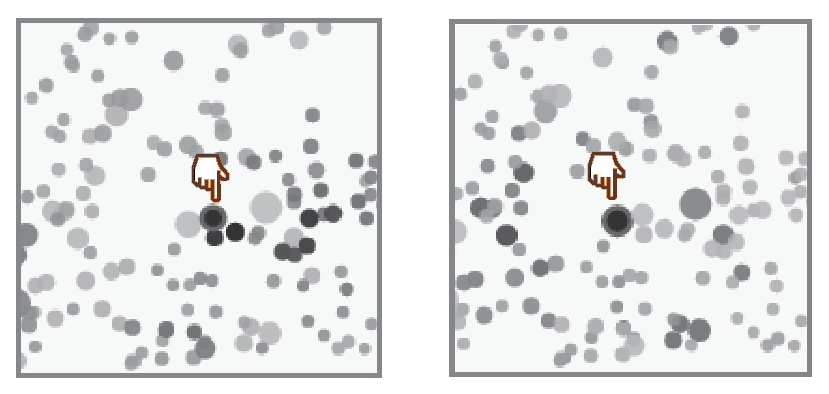
\includegraphics[width=0.65\linewidth]{images/suggestion_distortion.eps}
  \caption{Visualizing distortion with point size and color. When a datum is hovered, the saturation of other data reflect their high-dimensional distances to the hovered one. This image shows a case where two projection neighbors are probably far way in the high-dimensional space.}
\label{fig:enhancement_distortion}
  \end{figure}

In order to quantify distortions, we assess the accumulated distance errors for each datum:
\begin{equation}
Error(\mathbf{x}_{i}^{\prime}) = \sum\limits_{j=1}^{n}(Dist(\mathbf{x}_{i}, \mathbf{x}_{j})^{2} - Dist(\mathbf{x}_{i}^{\prime}, \mathbf{x}_{j}^{\prime})^{2}), i = 1,2,\cdots n
\end{equation}
  
Here $\mathbf{x}_{i}$ and $\mathbf{x}_{i}^{\prime}$ represents an high-dimensional datum and its projected counterpart. Distance is measured by the Euclidean metric. We use point size to show the distortion levels (Figure~\ref{fig:enhancement_distortion}). Larger points are more likely misplaced with 'false neighbors', that are projected nearby but actually far away in the high-dimensional space. When users hover on a datum, the saturation of other points change to reflect their high-dimensional distances to the hovered one. Closer data get higher saturation. This technique has also been used in~\cite{DBLP:journals/tvcg/StahnkeDMT16}. It allows users to find distorted datum / neighborhoods that may benefit a lot from local enhancements.
  
\note{
Lots of clustering algorithms can be applied to identify projection clusters~\cite{DBLP:conf/ieeevast/Kandogan12}. We adopt a variant of DBSCAN~\cite{zhou2012research} whose parameters are adaptive to the data. We choose DBSCAN because it can efficiently identify clusters in any shape. The self-adaptive parameters make it applicable to most datasets without the need of manual tuning. 


Refer to Figure~\ref{fig:suggestions}(b) for the effect of focus group suggestion. The potential clusters are shown as contours around the points. Users can choose any suggested cluster by simply clicking on it. To be clear, the suggestion only clarifies dominant relationships perceived by the user. It doesn't provide any extra information beyond the projection. If the user doesn't feel satisfied with the suggestion, he can choose his own focus by brushing the data.

For any given projection, we consider a datum interesting if its distances to other data have been severely distorted. To measure the distortion, we accumulate distance errors for each datum in the projection:

On the other hand, we provide interactive hints to reveal the real distances. The approach is similar to that used in~\cite{DBLP:journals/tvcg/StahnkeDMT16}, but uses a different metaphor. When user hovers on the projection, we construct a so-called 'high-dimensional lantern' using interpolation. Assume that the hovered position corresponds to a two-dimensional datum $\mathbf{p}^{\prime}$, we interpolate its high-dimensional counterpart as follows:
\begin{equation}
\mathbf{p} = \sum\limits_{i=1}^{n}\mathbf{w}_{i}\cdot\mathbf{x}_{i} =  \sum\limits_{i=1}^{n} \left (\frac{Dist(\mathbf{x}_{i}^{\prime}, \mathbf{p}^{\prime})^{-1}}{\sum\limits_{j=1}^{n}Dist(\mathbf{x}_{j}^{\prime}, \mathbf{p}^{\prime})^{-1}}\right )\cdot\mathbf{x}_{i}
\end{equation}
The interpolation weight $\mathbf{w}_{i}$ of data $\mathbf{x}_{i}$ depends on its distance to the hovered spot in the projection. Closer data get larger weights. When user hovers right on $\mathbf{x}_{i}^{\prime}$, $\mathbf{w}_{i}$ equals $1$ while all the other weights get $0$. The result equals to the original data: $\mathbf{p} = \mathbf{x}_{i}$.

By the interpolation, we aims to infer what kind of data is desired by the user. Then this desired point acts as a high-dimensional lantern, shedding lights on all the other data to indicate it distances to them. With the lighting metaphor, we encode distance information using the saturation tunnel in HSL color space:
\begin{equation}
\begin{split}
Saturation(\mathbf{x}_{i}^{\prime}) &= \max{\{(\alpha D_{i}^{2} + \beta D_{i} + \gamma)^{-1}, 1\}},\\
D_{i} &= Dist(\mathbf{x}_{i}, \mathbf{p}), \quad i = 1,2,\cdots n
\end{split}
\end{equation}
The data gets high saturation, if it's close to the interpolated point in the original space. The parameters $\alpha,\ \beta$ and $\gamma$ come from the inverse-square law of the lighting model. Empirical values are chosen to accommodate most datasets. Users can hover on any datum to check its neighborhood. If the neighborhood has been distorted, its lights will not be able to illuminate its neighbors in the projection. In contrast, the real neighbors will appear in far away places. Figure~\ref{fig:suggestions}(a) demonstrates a case, where two neighboring points cannot affect each other. They are probably false neighbors due to distortion.

In summary, large data points are potentially interesting data with high distortion and inconsistent illumination. With the hints, user hovers around the projection like experiencing an adventure. He holds a lantern to explore unknown structures in the complex data space. Compared to~\cite{DBLP:journals/tvcg/StahnkeDMT16}, this method enables a more smooth and natural perception of distance information.
}

\subsubsection{Focus Group Suggestion}
\label{subsection:groupsuggestion}
In a projection, we assume a group of data interesting if they appear as a cluster. Hence, we detect clusters in the projection and recommend them as potential POI groups.

\note{
Automatic clustering algorithms play an important role in previous works~\cite{DBLP:conf/ieeevast/NamHMZI07}~\cite{DBLP:journals/cgf/LeeKCSP12}~\cite{DBLP:journals/cgf/LiuWTBP15}. Users are either given the clustering results, or assisted in tuning parameters of the algorithm. However, it's not intuitive to drive the clustering by parameters, since the algorithm is often a black box to users. Besides, it's hard for users to understand causes and details about the clusters, let alone modifying them or discovering new ones.

In our method, we decide not to provide global clustering results. Instead, we suggest an interesting group of data by examining projection clusters. It is based on the fact that, no additional or prior knowledge should be assumed in a free exploration. Users choose their focuses based on what they perceive. We only reveal real structures of the chosen focus. Users can still take full control of the clustering process, after they get the local insights.}

Lots of clustering algorithms can be applied to identify projection clusters~\cite{DBLP:conf/ieeevast/Kandogan12}. We adopt a variant of DBSCAN~\cite{zhou2012research} whose parameters are adaptive to the data. We choose DBSCAN because it can efficiently identify clusters in any shape. It also reveals outliers in sparse regions. The self-adaptive parameters make it applicable to most datasets without the need of manual tuning. Refer to Figure~\ref{fig:suggestions}(b) for actual effects of the algorithm. Clusters are shown as contours around data points. Users can choose any suggested cluster by clicking on the contour.

Note that, either points or groups, we only make suggestions to guide and support users' decisions, not to replace them. Users can hide the suggestions at any time, and choose his own POI by brushing the desired data. All options are provided in Control Panel (see 'Focus' and 'Suggestion' in Figure~\ref{fig:teaser} ~(c)).


\subsection{Featured Projections of the Focus}
We call a chosen datum the focus point, and call a chosen group the focus group. After some focus is chosen, we generate projections to either reduce its distortion, or enhance its local features. The locally enhanced projection is updated in Projection View (Figure~\ref{fig:teaser}(a)) with highlighted POI data and grayed out contexts.

\subsubsection{Focus Point Enhanced Projection}
For a focus point, we assume that the user is interest in its high-dimensional neighbors. In other words, he may wish to find more data similar to the POI in different aspects. It's especially useful in scenarios where users start searching from a familiar case. For example, a college student longs for a good car but cannot afford the price. He can search for other cars with similar functions but at a lower price. In such case, mapping distortions could be a major obstacle. To reveal the true neighbors, we seek a projection to reduce overall distance distortions for the POI. Let $\mathbf{P}$ be the focus point, we aim to solve the following optimization problem:
\begin{equation}
\begin{split}
\min Error(\mathbf{P}) &= \min_{\mathbf{A}}  \sum\limits_{i=1}^{n}(Dist(\mathbf{P}, \mathbf{x}_{i})^{2} - Dist(\mathbf{PA}, \mathbf{x}_{i}^{\prime})^{2})\\ 
s.t.\ \mathbf{A^{T}A} &= \mathbf{I}
\end{split}
\end{equation}
Here the term $\mathbf{A}$ represents a projection matrix containing unit vectors, and $\mathbf{I}$ is the identity matrix. The projected focus is $\mathbf{P^{\prime}} = \mathbf{PA}$. What we do via the optimization is that, we push away all 'false neighbors' that are far from POI in the high-dimensional space. The mapped neighborhood is then left with real neighbors. Since the high-dimensional distances are invariant between POI and other data, the term $Dist(\mathbf{P}, \mathbf{x}_{i})^{2}$ is simply a constant. The minimization problem can be written in the following form:
\begin{equation}
\label{equation:center-shiftedPCA}
\max_{\mathbf{A}}  \sum\limits_{i=1}^{n}Dist(\mathbf{PA}, \mathbf{x}_{i}^{\prime})^{2},\ s.t.\ \mathbf{A^{T}A} = \mathbf{I}
\end{equation}
Note that if we replace $\mathbf{P}$ with the mean data $\mathbf{\bar{x}}$, the optimization will directly lead to PCA projection in Euclidean distances. In other words, the locally enhanced projection can be regarded as PCA with a shifted center (i.e. the chosen focus). Thus the optimization is no harder than a simple PCA algorithm. Accelerating skills for PCA are also applicable to speed up the optimization.
\note{
This center can reach its lowest distortion level. In turn, PCA can be thought of a single-datum distortion reduction. It lowers the overall distortion level, by helping the average datum. Figure~\ref{fig:car}(c) demonstrates the actual effect of our center-shifted PCA. As a result, the other data have more accurate distances towards the focus. False neighbors will be pulled away, leaving a more authentic neighborhood around the focus.
}

Compared to the direct distance correction used in~\cite{DBLP:journals/tvcg/StahnkeDMT16}, our method preserves all benefits of a linear projection rather than mere point-wise distances. It provides rich dimensional context, and help maintain a consistent mental model of the data space. In Section~\ref{subsubsection:relationship_enhancement}, we will further integrate this projection into a larger framework.
\note{interpret this projection in the context of data relationships.}

\subsubsection{Featured Local Relationships}
For a focus group, we first examine what kinds of features are of interest in the local analysis. By features, we refer to featured relationships related to the focus group, such as sub-grouping, outliers, etc. Since relationships are defined based on distances, we can take a look at the distance matrix. Given the POI group, the whole distance matrix is divided into three parts (Figure~\ref{fig:local_relationships}(a)). The first part describes distances between group members. The second part is about distances between the group and the other data. The last part describes distances among the context data. Since the last part has nothing to do with the focus, we simply ignore it. For the remaining parts, we consider the data to be either 'similar' or 'dissimilar' (Figure~\ref{fig:local_relationships}(b)).

By revealing similarities among group members, we can show users in which aspects the data are most similar. It helps to comprehend why these data gather into a cluster in the projection. Enhancing dissimilarities, on the other hand, tells about the major differences among group members. If there are sub-clusters within the group, their differences will be more prominent when enhanced. It helps to reveal hidden local structures.

Currently, we did not consider similarities between the group and the others. It's based on the fact that, we'll have to distinguish between two parts before talking about their similarities. If we ignore the differences, similarity between two complementary parts is always equal to similarities among all data, i.e. the inter-group similarity of the whole dataset. In that case, there is no need for such setting. In contrast, by enhancing the dissimilarities, we can show why the focus group is different from the others. The idea resembles that of Linear Discriminant Analysis (LDA), expect that we did not regard the other data as a same class.

In summary, three types of relationships are found most informative in the local analysis. We call them intra-group similarity, intra-group dissimilarity and inter-group dissimilarity respectively (Figure~\ref{fig:local_relationships}(b)).

\begin{figure}[htbp]
\centering
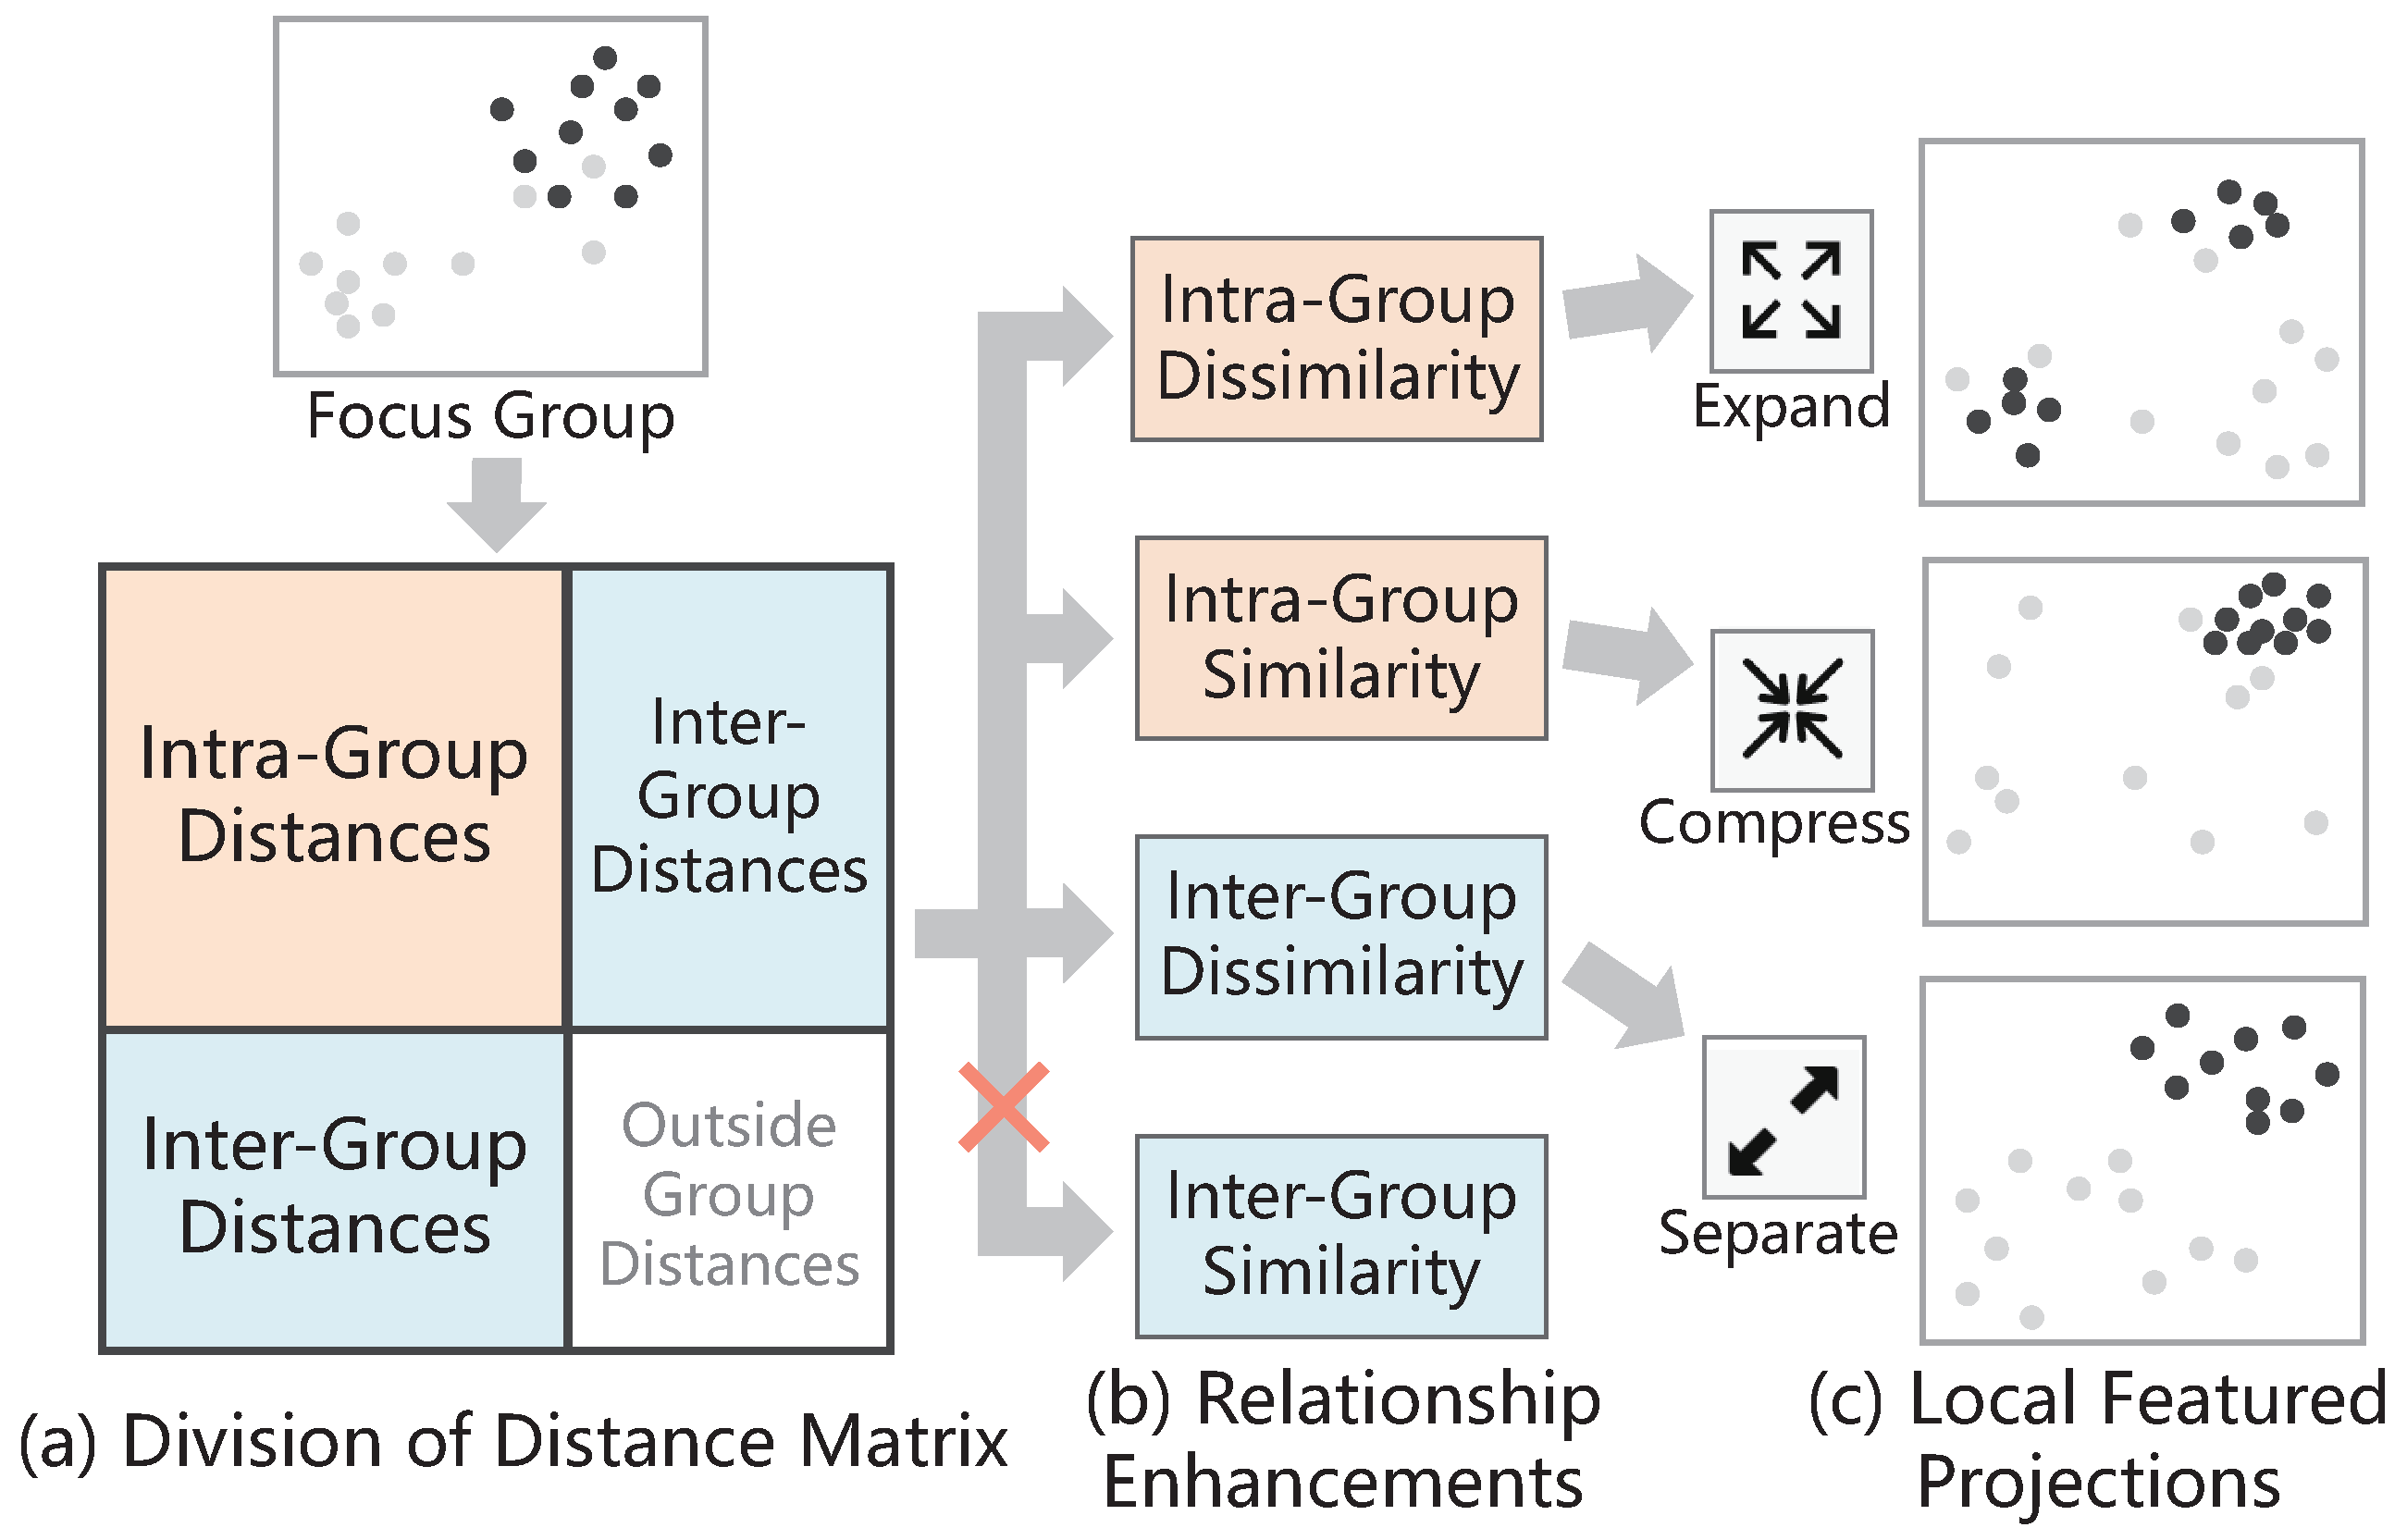
\includegraphics[width=1\linewidth]{images/enhancement1.eps}
  \caption{Enhancing featured local relationships. Given a focus group, the distance matrix is divided into three parts~(a). We enhance data similarity / dissimilarity based on each part~(b). Three types of projections are generated via the local enhancements~(c).}
\label{fig:local_relationships}
  \end{figure}

\subsubsection{Focus Group Enhanced Projections}
\label{subsubsection:relationship_enhancement}
With the three types of relationships, we first translate them in the language of data distances. Then we adopt projection pursuit to find linear projections for the enhancement.

Enhancing similarities or dissimilarities, equals to decreasing or enlarging data distances in the projection. For a focus group $G$, we enhance the intra-group dissimilarities by:
\begin{equation}
\begin{split}
\max \sum\limits_{\mathbf{x}_{i}^{\prime}, \mathbf{x}_{j}^{\prime} \in G} Dist(\mathbf{x}_{i}^{\prime}, \mathbf{x}_{j}^{\prime})^{2} &= \max_{\mathbf{A}} \sum\limits_{\mathbf{x}_{i}, \mathbf{x}_{j} \in G} Dist(\mathbf{x}_{i}\mathbf{A}, \mathbf{x}_{j}\mathbf{A})^{2}\\ 
s.t.\ \mathbf{A^{T}A} &= \mathbf{I}
\end{split}
\end{equation}
  
For simplicity, we call this optimization the \textbf{Expand} metric, since the focus group will be expanded in the resulting projection. It actually leads to a local PCA projection (see Appendix). Likewise, we enhance the similarities by minimizing the same metric:
\begin{equation}
\min_{\mathbf{A}} \sum\limits_{\mathbf{x}_{i}, \mathbf{x}_{j} \in G} Dist(\mathbf{x}_{i}\mathbf{A}, \mathbf{x}_{j}\mathbf{A})^{2},\ s.t.\ \mathbf{A^{T}A} = \mathbf{I}
\end{equation}
  
We call it the \textbf{Compress} metric, as the opposite of Expand. At last, we enhance the inter-group dissimilarities by enlarging distances between the group and the other data:
\begin{equation}
\label{equation:Separate}
\max_{\mathbf{A}} \sum\limits_{\mathbf{x}_{i} \in G} \sum\limits_{\mathbf{x}_{j} \in \bar{G}} Dist(\mathbf{x}_{i}\mathbf{A}, \mathbf{x}_{j}\mathbf{A})^{2},\ s.t.\ \mathbf{A^{T}A} = \mathbf{I}
\end{equation}
This one is called the \textbf{Separate} metric. We use glyphs to denote different feature enhancements throughout the whole system. Figure~\ref{fig:local_relationships}(c) illustrates those glyphs, as well as projections generated from different metrics. User can change the enhanced feature in the Control Panel (see 'Features' in Figure~\ref{fig:teaser} (c)), regarding the analytic task at hand.

In fact, we can see a focus point as a group containing only one datum. There will not be Compress or Expand projections, but the Separate metric simply degrades to the center-shifted PCA (compare equation~(\ref{equation:center-shiftedPCA}) and~(\ref{equation:Separate})). This enables us to combine all featured projections into the same framework.

At last, solutions to all optimization problems can be approximated via eigen-decompositions in \textbf{O}($D^3$) time (see Appendix), with D being the number of dimensions. The complexity can be further reduced by numerical techniques. It makes our method well scalable to larger datasets with higher dimensions.

\subsubsection{Subspace Suggestion}
When pursuing the feature enhanced projections, we take into account all dimensions. However, only a few of them truly contribute to the features. Redundant dimensions will obscure the patterns and interfere with dimensional analysis. Hence, we need to reveal a feature-related subspace to promote subsequent analysis.

In a sense, projection pursuit itself is a process to identify the most featured dimensions. Based on its results, we can make reliable judgements on dimension contributions. To be specific, we first generate an enhanced projection with all dimensions considered. Then we examine dimension weights in that projection, and rank all dimensions by their weights: $W(d_{1}^{*}) > W(d_{2}^{*}) > \cdots >W(d_{m}^{*})$. All weights are normalized and sum to 1. At last, we pick out dimensions with large weights, until their sum exceeds a certain threshold:
\begin{equation}
\begin{split}
&Subspace = \{d_{i}^{*}| i = 1,2, \cdots L \},\\
&s.t.\ \sum\limits_{j=1}^{L} W(d_{j}^{*}) \leq R \ \text{and}\ \sum\limits_{j=1}^{L+1} W(d_{j}^{*}) > R
\end{split}
\end{equation}
Threshold $R$ is set as 0.75 by default, cutting down at least $25\%$ redundant dimensions. That gives us a subspace most related to the enhanced feature. The sum of weights is called \textbf{Subspace Score}. It indicates how strong the chosen subspace is related to the current feature. \note{In fact, it is the same strategy as rank-by-feature~\cite{DBLP:journals/ivs/SeoS05}, except that our feature scores are dimension weights of a featured projection.} Dimension weights are always displayed as a bar chart in the Information Panel (Figure~\ref{fig:teaser} (b)). Users can include / exclude dimensions by brushing in this view.

After gaining a subspace, we run optimizations again in that subspace to get the final result. The refined projection will be easier to interpret with only the most related dimensions. Features will also be more prominent.

\note{related to rank-by-feature}

\subsection{Modifying the Focus}
For a focus point, a distortion reduced projection is the final step. But for a focus group, it still needs to be modified. The featured projections support this task by revealing local insights.

The Expand projection shows minor relationships hidden in the group. It reveals sub-clusters and outliers, and helps to trim the POI into a more consistent group. The Compress projection enhances similar aspects within the group. If there are other data that resemble the focus in such aspects, they will also be drawn closer to the group, claiming to be potential members. It helps to regain the missing members. The Separate projection highlights differences between group members and the others. Boundary points will stand out in this case, which helps to clarify cluster boundaries.\note{The above benefits largely owe to the combination of local optimization and focus + context technique. In previous works with only local projections~\cite{DBLP:journals/tvcg/YuanRWG13}, it's hard to modify a focus without any context information.}

We support the modification by providing focus-aware brushing techniques (see 'Selection' in Figure~\ref{fig:teaser} (c)), in order to avoid interference from the context. When user needs to add more members, he can use the 'Increase' brush. Whatever chosen by the brush will be added into the current focus group. When there is a need for decreasing members, the 'Decrease' brush can be used. Intersection of the current group and the brushed data will be chosen as the new focus.

Once the focus group is changed, the projection will also be updated. Smooth transitions are applied to avoid swift changes (see the supplementary video). We keep an orthogonal mapping in each frame of the transition~\cite{cook2004computational}, so as to maintain an intact mental model of the high-dimensional data structure.

\subsection{Storing and Comparing Multiple Focuses}
During the exploration, there will be times when users need to store the results. For example, when sub-groups are found, the current group shall be stored before focusing on a smaller group. Besides, there are needs to compare different focuses regarding their features. We provide the \textbf{Focus List} and the \textbf{Projection Map} to support such tasks.

In the Focus List (Figure~\ref{fig:teaser} (d)), users can store the current focus or retrieve a previous one. Each focus is represented as a node. Its size denotes the data size, while colors differentiate different focuses. When hovering on a node, users can name the focus or change its color. Specially, there is a fixed node called 'All Data'. Enhancing its Expand feature will lead to a global PCA projection.

For every focus in the list, its enhanced projections for all three features are shown as glyphs in the Projection Map (Figure~\ref{fig:teaser} (e)). Different glyphs denote different features (Figure~\ref{fig:local_relationships} (c)). Dimension weights are displayed as small histograms on top of each glyph to help compare the projections. Clicking on a glyph can retrieve the focus and corresponding projection.

To measure similarity between projections, we refer to the manifold learning domain. It has been proved that any two 2D projections lie on the same Grassmann manifold. Their dissimilarity can thus be measured by their geodesic distance on this manifold~\cite{absil2004riemannian}. We choose this metric since it reflects dimensional diversity between projections, which is important in feature comparison. After gaining the distances, we construct the final map using MDS algorithm. Due to the mapping technique, there may be occlusions between glyphs. Nevertheless, users can always clarify the clutter by hovering on a focus node, which can highlight related glyphs in the map.

\note{
In the projection map, users can compare features of different focuses. For example, two focus groups may have the same reasons for the grouping (i.e. intra-group similarities), while having different inner-group diversities (see Figure~\ref{fig:map}). It helps to understand different local data in the context of featured dimensions. In addition, users can plan their own high-dimensional tours in this map. A similar idea has been proposed in the TripAdvisor~\cite{DBLP:journals/tvcg/NamM13}, as an extension of the Grand Tour~\cite{asimov1985grand}~\cite{cook1995grand}. But their projections are driven by dimensions without explicit semantics. In comparison, each spot in our map is tightly related to some local data and a certain relationship. It makes the tour more targeted and easier to interpret.
}